\section{\MBSim - Program Overview}
\MBSim{} is written in the object-orientated programming language C++. 

Fig.~\ref{fig:objects} shows a class diagram.
\begin{figure}
	\centering
  	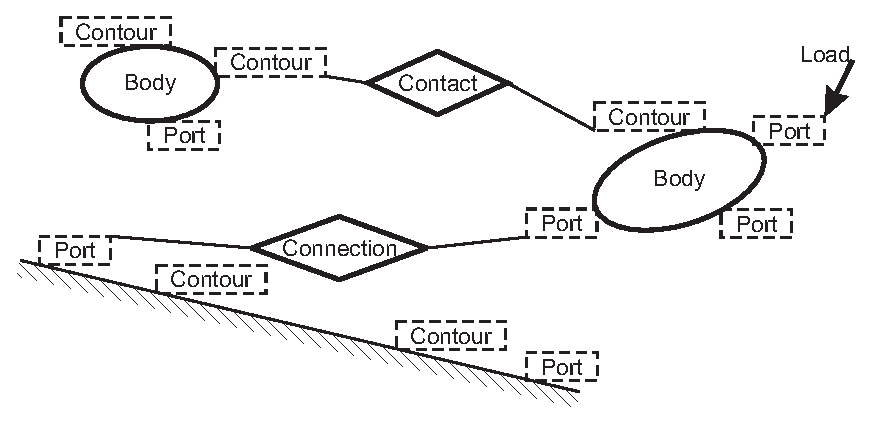
\includegraphics[width=12cm]{Figures/objectorientationMBSim.eps} % TODO
  	\caption{object structure in \MBSim}
  	\label{fig:objects}
\end{figure}

\subsection{Description of the Components}

\subsection{Program Flow}
Conceptionally the program flow is defined by the election of the integration scheme.

\subsubsection{Timestepping Integration}
Timestepping integration solves the whole equations of the system including the contacts on velocity level with fixed time step size. In detail one has the following work flow.
\begin{enumerate}
\item $\text{\texttt{DS::plot}}\left(t,\vq,\vu\right)$
\item $\vq\leftarrow\vq+\text{\texttt{DS::deltaq}}\left(t,\vq,\vu\right)$
\item $t\leftarrow t+\Delta t$
\item $\text{\texttt{DS::update}}\left(t,\vq,\vu\right)$
    \begin{enumerate}
    \item[]\texttt{DS::updateStateDependentVariables}\\
      update variables depending on the generalised state and the structure of the system with one independent group and several trees
    \item[]\texttt{DS::updateg}\\
      \begin{itemize}
      \item update of the relative position kinematics independent of the system structure using the order
      \begin{align*}
        \text{\texttt{Link}}\rightarrow\text{\texttt{LinkMechanics}}\rightarrow\text{\texttt{Joint}, \texttt{Contact}, \texttt{Actuator}}\rightarrow\text{\texttt{ContactKinematics}}
      \end{align*}
      \item several contacts points are possible from the kinematical point of view, whereby the maximum number is calculated in \texttt{ContactKinematics}\\
      \item conventions in the contact frame matrix:
        \begin{itemize}
        \item frames are cartesian
        \item first column is the outpointing normal
        \item second column sign is different for the two contacting bodies 
        \end{itemize}
      \end{itemize}
    \item[]\texttt{DS::checkActiveg}\\
      \begin{itemize}
      \item determine the state of the relative kinematics concerning the activity of links
      \item redefine global memory references using indices and indents
      \end{itemize}
    \item[]\texttt{DS::updategd}\\
      \begin{itemize}
      \item update of the relative velocity kinematics independent of the system structure
      \item can be done in the child classes of \texttt{LinkMechanics}
      \end{itemize}
    \item[]\texttt{DS::updateT}\\
      updates the linear transformation matrix $\dot{\vq}=T\vu$ independent of the system structure
    \item[]\texttt{updateJacobians}\\
      updates
    \end{enumerate}
\item $\text{\texttt{DS::solveImpacts}}\left(t,\vq,\vu\right)$
\item $\vu\leftarrow\vu+\text{\texttt{DS::deltau}}$
\item $\vx\leftarrow\vx+\text{\texttt{DS::deltax}}$
\item \texttt{DS::projectGeneralizedPositions}
\end{enumerate}

\subsubsection{Event-Driven Integration}

%exemplarisch ein System aus Umwelt und zwei K�rpern. Angedeutet sind Wechselwirkungen
%dieser untereinander �ber Kontakte und Verbindungen sowie eine �u�ere Last.
%
%Ein K�rper~(\texttt{Body...}) ist in \MBSim{} durch seine Lagen~$\vq$ und
%Geschwindigkeiten~$\vu$ parametrisiert. Die Parameter der beschreibenden
%Differentialgleichung sind bei starren K�rpern~(\texttt{BodyRigid...}) immer Masse~$m$ und
%Tragheitstensor~$\vTheta$. Die Modelle f�r flexible K�rper~(\texttt{Bodyflexible...}) sind in der
%Parametrisierung jeweils sehr speziell -- f�r sie sei auf die jeweiligen Implementierungen
%und die zugeh�rigen Dokumentationen verwiesen.
%
%Die Umwelt kann wie auch alle K�rper Konturen~(\texttt{Contour}) sowie
%Anschl�sse~(\texttt{Port}) aufnehmen, auf denen Kontakte sowie diskrete Wechselwirkungen
%definiert werden k�nnen. Zudem ist Gravitation �ber die Umwelt definiert.
%
%Kontakte zwischen den Konturen unterschiedlicher K�rper k�nnen sowohl als
%Starrk�rperkontakt~(\texttt{ContactRigid}, mengenwertig, nicht-glatte Dynamik) als auch
%als nachgiebiger Kontakt~(\texttt{ContactFlexible}, funktional, lokale Steifigkeit)
%definiert werden. Reibung wird hierbei jeweils durch die Angabe der auszuwertenden
%Reibrichtungen eingebunden. Verbindungen zwischen zwei Anschl�ssen k�nnen sowohl starr
%(\texttt{ConnectionRigid}) als auch mit Nachgiebigkeit~(\texttt{ConnectionFlexible})
%modelliert werden. F�r �ussere Lasten~(\texttt{Load}) k�nnen beliebige Vorschriften
%angegeben werden.
%%------------------------------------------------------------ SUBSECTION --
%\subsection{M\"oglichkeiten der Modellierung}
%Bei der Modellierung in \MBSim{} kann auf folgende Klassen des Kernes
%zur\"uckgegriffen werden. Weitere Klassen werden unter anderem in \texttt{mbsimAddOn} zur Verf\"ugung
%gestellt.
%
%\subsubsection{Starr-K\"orper}
%\begin{itemize}
%\item \emph{BodyRigidAbs} f\"ur Definition von Starrk\"orpern gegen\"uber einem Inertialsystem
%\item \emph{BodyRigidRel} f\"ur Definition von Starrk\"orpern gegen\"uber einem Vorg\"angersystem
%\item \emph{BodyRigidConstrainedAcc} f\"ur Starrk\"orper mit vorgegebener Beschleunigung gegen\"uber einem Inertialsystem (Tr\"agheiten werden hierbei nicht ber�cksichtigt)
%\item \emph{BodyRigidConstrainedVel} f\"ur Starrk\"orper mit vorgegebener Geschwindigkeit gegen\"uber einem Inertialsystem (Tr\"agheiten werden hierbei nicht ber�cksichtigt)
%\item \emph{BodyRigidRelonFlex} erster Starrk\"orper, der auf flexiblen K\"orper gesetzt wird
%\item \emph{TreeRigid} f\"ur die Zusammensetzung von \emph{BodyRigidRel}
%\end{itemize}
%In jedem Fall sind Masse (\emph{setMass}), Tr\"agheitstensor bez. dem Bezugspunkt (\emph{setInertia}), generalisierte Koordinaten (\emph{setJT}, \emph{setJR}), evtl. Anfangsverformungen (\emph{setWrOK0}, \emph{setAWK0}) und \AMVis{}-Darstellungen (\emph{setAMVisBody}) anzugeben und die K\"orper dem MKS hinzuzuf\"ugen (\emph{addObject}). Auch ganze MKS k\"onnen als Slave einem Master-MKS hinzugef\"ugt werden.
%
%\subsubsection{Flexible-K\"orper}
%\begin{itemize}
%\item \emph{BodyFlexible1s01Torsion}
%\item \emph{BodyFlexible1s21ANCF} 2D-Balken mit Absolute Nodal Coordinate Formulation
%\item \emph{BodyFlexible1s21RCM} 2D-Balken mit Redundant Coordinate Method (3-Koordinaten pro Knoten $x$, $y$, $\gamma$ und 2 zus\"atzliche Koordinaten pro Balken $c_1$, $c_2$)
%\item \emph{BodyFlexible1s23BTA} Biege-Torsions-Welle (5-Koordinaten pro Knoten $\alpha$, $y$, $\gamma$, $z$, $\beta$ im jeweils mit $\alpha$ mitdrehenden KOSY)
%\item \emph{BodyFlexibleLinearExternal}
%\item \emph{TreeFlexRoot} f\"ur die Zusammensetzung eines flexiblen K\"orpers und eines Starrk\"orpers 
%\end{itemize}
%F\"ur die RCM-Modelle sowie die Biege-Torsions-Welle kann eine \AMVis-Darstellung
%(\emph{createAMVisBody}) aktiviert werden. Die Finiten Elemente selbst basieren im Fall von \emph{BodyFlexible1s21RCM}, \emph{BodyFlexible1s23BTA} und \emph{BodyFlexibleLinearExternal} auf einem neugeschaffenem Interface \emph{DiscretizationInterface} zur einheitlichen Darstellung.
%
%\subsubsection{Verbindungen}
%Verbindungen werden ohne Reibung \"uber Ports (\emph{addPort}, \emph{connect}) an K\"orper bez. an die Umgebung angeschlossen. Dann ist auszuw\"ahlen, ob eine flexible Verbindung (\emph{ConnectionFlexible}) oder eine Starrk\"orperverbindung (\emph{ConnectionRigid}) zwischen K\"orpern oder eine externe Erregung (\emph{Load}) zur Modellierung verwendet werden soll. Der Freiheitsgrad der Verbindung wird \"uber \emph{setForceDirection} bez. \emph{setMomentDirection} angegeben. Dem MKS wird eine Verbindung anschlie"send \"uber \emph{addLink} mitgeteilt. \"Uber \emph{Link} kann auch eine Visualisierung der Verbindungskr\"afte (\emph{Arrow}) und der Kopplung selbst zugeschaltet werden; hierbei ist es m\"oglich zwischen einer Einheitenumrechnung und einer L\"angenvisualisierung zu unterscheiden (\emph{setScaleFactor}, \emph{setArrowHead}, \emph{setDiameter}), sowie den Partner f\"ur das Pfeilende festzulegen. Bei \emph{Load} wird mit \emph{setSignal} eine benutzerspezifische Funktion\footnote{\emph{UserFunction} gibt es bereits mit harmonischen (\emph{FuncHarmonic}), linearen Verlauf (\emph{FuncLinear}), oder auch als mehrdimensionale st\"uckweise Polynominterpolation (\emph{MDPPolynom})} vorgegeben.
%
%\subsubsection{Kontakte und St\"o"se}
%Kontakte und St\"o"se (\emph{Contact, ContactBilateral, Impact}\footnote{Vorsicht bei gleichzeitiger Modellierung von Reibung: es k\"onnen Widerspr\"uche zwischen Energieerhaltung in normaler Sto"srichtung und Dissipation durch Reibung auftreten.}) werden K\"orpern \"uber
%passive Konturen (\emph{addContour}, \emph{connect}) und aktive Kraftgesetze
%hinzugef\"ugt. Die Zahl der Reibrichtungen und -parameter muss hierbei explizit angegeben werden
%(\emph{setFrictionDirections}, \emph{setFrictionCoefficientFunction}). Bei einem Sto"s muss
%zus\"atzlich der Sto"skoeffizient (\emph{setNormalRestitutionCoefficient}) angegeben
%werden, der beim Kontakt $0$ gesetzt wird. Dem MKS wird ein Kontakt bez. Sto"s
%anschlie"send \"uber \emph{addLink} mitgeteilt.\\
%Die Kontakt-Konturen sind so zu w\"ahlen, dass die Schnittmenge der beteiligten Kontakt-/
%Sto"skonturen maximal einpunktig ist. Implementiert sind derzeit die Konfigurationen
%Punkt-Linie, Punkt-Ebene, Punkt-Kante, Punkt-Polytop, Punkt-Zylinder, Punkt-Contour1s,
%Punkt-Kegelstumpf, Punkt-Interpolationskontur, Kreis-Contour1s, Kreis-Linie, Kreis-Ebene,
%Kreis-Kreisinneres, Kreis-Kreis, Kreis-Kegelstumpf, Kreisinneres-Zylinder,
%Linie-Contour1s, Kugel-Ebene, Kugel-Kugel und Kugel-Kegelstumpf. Auch Erweiterungen
%k\"onnen \"uber die Definition neuer Konturen und zugeh\"origer Kontaktkinematiken
%(\emph{setContactKinematics}) definiert werden. Hierzu ben\"otigt eine Kontur die
%Parametrisierung einer nach innen gerichteten Normale, einer Tangente, einer Position,
%einer Geschwindigkeit und einer Winkelgeschwindigkeit. Die Kontaktkinematik muss in einem
%ersten Schritt Normalabstand und Konturparameter \"uber eine Nullstellenfunktion
%bestimmen, sowie tangentiale Richtungsinformationen f\"ur Reibung in einem zweiten
%Schritt. Die Reihenfolge des \emph{connect}-Aufrufs muss dar\"uberhinaus behandelt
%werden.
%
%\subsubsection{Integratoren}
%Bei Integratoren stehen \emph{DOPRI5Integrator} f\"ur nichtsteife ODE- und \emph{RADAU5Integrator} f\"ur steife ODE-Systeme zur Verf\"ugung; DAEs behandeln \emph{RADAU5DAEIntegrator}, \emph{DASKRIntegrator} und \emph{DASPKIntegrator}. Alle arbeiten mit Schrittweitensteuerung. Dar\"uberhinaus gibt es noch \emph{RKSuite}, \emph{LSODAR} (Mehrschrittverfahren steif/nicht steif) und \emph{LSODE}. Bei Ungleichungsnebenbedingungen muss der semi-implizite \emph{TimeSteppingIntegrator} oder der allgemeinere \emph{ThetaTimeSteppingIntegrator} mit konstanter Schrittweitenvorgabe angewendet werden. \emph{TimeSteppingSSCIntegrator} implementiert f�r den semi-impliziten Fall eine Schrittweitensteuerung und \emph{DAETSIntegrator} liefert eine Kopplung zwischen TimeStepping und Dassl. Bei letzteren muss der Befehl \texttt{setSolver} vor der Initialisierung des MBS durchgef\"uhrt werden. Folgende M\"oglichkeiten stehen zur Wahl:
%\begin{itemize}
%\item Invertierbare Gleichungssysteme (GS) mit nur bilateralen Bindungen\\
%\emph{LinearEquations}: Cholesky-Verfahren
%
%\item St\"uckweise Lineare GS (2D-Coulomb-Reibung)\\
%\emph{GaussSeidel}: Gauss-Seidel-Verfahren
%
%\item Nichtlineare GS (3D-Coulomb-Reibung)\\
%\emph{FixedPointSingle}: Gauss-Seidel-Verfahren mit Fixpunktsuche und R-Faktor-Strategie
%  (\emph{setStrategy} mit \emph{local}/\emph{global})\\
%\emph{FixedPointTotal}: Jacobi-Verfahren mit Fixpunktsuche und R-Faktor-Strategie (verh\"alt sich zumeist schlechter als \emph{FixedPointSingle})\\  
%\emph{RootFinding}: ged\"ampftes, z.B durch Regula Falsi generalisiertes Newton-Verfahren mit
%  R-Faktor-Strategie (unstetige Jacobi-Matrix) und f\"ur unterbestimmte LGS ausw\"ahlbarer \emph{setLinalg} (LUDecomposition, LevenbergMarquardt, PseudoInverse) (f\"ur schlecht konditionierte Dylassus-Matrix meistens am besten)
%\end{itemize}
%Der Befehl \emph{stopifnoConvergence(\texttt{true},\texttt{true})} zwingt den Integrator abzubrechen, falls keine Konvergenz vorliegt, und die Kontaktsituation auszugeben.
%
%%%------------------------------------------------------------ SUBSECTION --
%\subsection{Hinweise}
%\begin{enumerate}
%  \item F\"ur Anwendungen die MBSim-Ableitungen verwenden, muss im \texttt{Makefile} der
%       \texttt{pkg}-Aufruf ge\"andert werden zu \texttt{mbsimMechAdd} oder Adequates, um
%       die Bibliotheken einzubinden.
%  \item In \emph{Vec}-Schreibweise d\"urfen nur Ziffern auftreten
%  \item Parametrisierung der Gesamtbewegung (siehe Skriptum \cite{Foer07}) mit $\vA_{K_0K}$ durch $\vq$ und mit direkt vorgebbarem $\vA_{WK_0}$
%  \item Plotlevel (0,1,2,3) erh\"oht f\"ur jedes Element extra die Ausgabedateigr\"o"se (z.B. zus\"atzlich Kontaktgeschwindigkeiten); f�r AMVis ist ein Wert gr��er als 0 n�tig.
%  \item Projektionen zur Korrektur bei Verletzung von Lage-Nebenbedingungen sind bei Time-Steppern \"uber \emph{setDriftCompensation} m\"oglich. Bei der Interpretation ist
%       allerdings der Drift vom Diskretisierungsfehler (Time-Stepper ist 1. Ordnung) zu
%       unterscheiden; bei Kontaktdurchsinken sollte demnach zun\"achst die Schrittweite
%       verkleinert werden. Bei h\"ochstens Gleichungsnebenbedingungen k\"onnen bei reinen
%       Starrk\"orpersystemen auch alle anderen
%       Integratoren verwendet werden, da das System dann intern auf Beschleunigungsebene gebracht
%       wird, bei flexiblen K\"orpern ist dies nur zum Teil der Fall. Auch f\"ur Integratoren
%       h\"oherer Ordnung entsteht also ein numerischer Drift. Zur Vermeidung von numerischen
%       Fehlern ist es h\"aufig besser, Gleichungsnebenbedingungen
%       durch relativkinematische Beschreibungen zu ersetzen.
%  \item Es besteht die M\"oglichkeit von negativen Abst\"anden bis zur Kontaktdetektion, da die Kontakte mit Toleranzen versehen sind (zur Behebung ist die Schrittweite manuell zu verringern).
%  \item Bei unterbestimmten GS sind Kr\"afte au"serhalb der Bewegungsebene m\"oglich, solange die Physik nicht verletzt wird. Eine Addition aller Kr\"afte ergibt hierbei die korrekte Gesamtkraftwirkung. Alternativ k\"onnen \emph{flexibleLinks} oder z.B. bilaterale Links verwendet werden, die passive Kr\"afte eindeutig berechnen. Die Modellierung in MBSim ist im Wesentlichen gleich, jedoch kann dann wieder das Newton-Verfahren mit LU-Zerlegung als Solver benutzt werden. Z.B. im Reibungsfall sind solche alternativen Modellierungen zur Vermeidung mathematischer Abh\"angigkeiten nicht m\"oglich. Hier muss also ein iterativer L\"oser verwendet werden. Eine Konvergenzanalyse ist dann allerdings nicht m\"oglich.
%  \item Standardm\"assig werden die Kontaktkr\"afte nur im aktiven Fall aktualisiert, um den Vorg\"angerwert zur schelleren Konvergenz auszunutzen. Mit \emph{setUseOldla} kann dies unterbunden werden.
%  
%  \item Kontakte m\"ussen f\"ur jeden K\"orper extra definiert werden, um die Physik jeweils gleich zu behandeln.
%  \item Der Zustand kann f�r \emph{Tree} derzeit nicht ausgegeben werden.
%\end{enumerate}

%%------------------------------------------------------------ SUBSECTION --
\subsection{Plot Routines}\label{sec:plot}

\subsubsection{Usage}
For getting data from \MBSim{} a \HDF{} wrapper is used. Viewing the multibody system parts can be done with
\begin{verbatim}
    h5lsserie <h5-file>
\end{verbatim}
Several possible options are explained by typing \texttt{-h}:
\begin{enumerate}
\item[\texttt{-d}] shows the description of the data to plot\\
\item[\texttt{-l}] shows the column labels of the data to plot\\
\item[\texttt{-f}] follows external links in a set of \HDF{}-files to avoid redundant data (\HDF{} is possible per DynamicSystem)
\end{enumerate}
The specific names in \HDF{} format are specialised by reading from right to left. The url to specific data is given by a path and can be used in
\begin{verbatim}
    h5dumpserie <path>
\end{verbatim}
The column one is interested in is declared using a colon. Also several columns can be appended, whereby shorter ones are enlarged by \texttt{nan} entries. Altogether, it is possible to use the dump by
\begin{verbatim}
    gnuplot "<dump" u *:* w l
\end{verbatim}
or in \textsf{MatLab} by
\begin{verbatim}
    h5dump('<path>')
\end{verbatim}

\subsubsection{Implementation}
In \MBSim{} plotting is done using \texttt{plotFeatures} being defined in \texttt{element.h} and set in \texttt{multi\_body\_system.cc}. One plot-file comprises time-series of rowvectors with the same data type in all entries.

